\documentclass[convert={imagemagick, density=1024}]{standalone}
\usepackage{amsmath, amsthm, amsfonts,xcolor,pgfplots}
\usepackage{tikz-cd, kotex}
\usetikzlibrary{decorations.markings}
\usetikzlibrary{3d,intersections}
\usepgfplotslibrary{colorbrewer}
\usepackage{../.preamble/quiver}
\usepackage{../.preamble/Operators}
\begin{document}
\nopagecolor




\end{document}










\begin{tikzpicture}
  \draw[blue, -{stealth}] (-1,0) -- (.1,0);
  \draw[blue] (-1,0) -- (1,0);
  \fill[red] (-1,0) circle[radius=1pt];
  \fill[red] (1,0) circle[radius=1pt];
  \draw (-1,0) node[below]{$v_0$};
  \draw (1,0) node[below]{$v_1$};
  \draw (0,0) node[above]{$a$};
  \begin{scope}[shift={(3,0)}]
    \fill[orange, opacity=.2] (0,0) cihrcle[radius=1];
    \draw[-{stealth}, blue] (90:1) arc (90:150:1);
    \draw[blue] (149:1) arc (149:210:1);
    \draw[-{stealth}, blue] (210:1) arc (210:270:1);
    \draw[-{stealth}, blue] (269:1) arc (269:275:1);
    \draw[blue] (274:1) arc (274:330:1);
    \draw[->, blue] (90:1) arc (90:30:1);
    \draw[blue] (31:1) arc (31:-30:1);
    \fill[red] (90:1) circle[radius=1pt] node[above, black]{$v_0$};
    \fill[orange] (210:1) circle[radius=1pt] node[below left, black]{$v_1$};
    \fill[purple] (330:1) circle[radius=1pt] node[below right, black]{$v_2$};
    \draw (150:1) node[above left]{$c$};
    \draw (270:1) node[below]{$b$};
    \draw (30:1) node[above right]{$a$};
  \end{scope}
\end{tikzpicture}


%% Simplices (Homology-1.png)
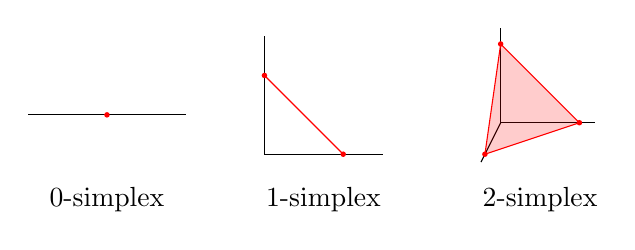
\begin{tikzpicture}
\draw (0, -.7)--(2,-.7);
\fill[red] (1,-.7) circle[radius=1pt];
\draw (1,-1.5) node[below] {$0$-simplex};

\draw (3,-1.2)--(4.5,-1.2);
\draw (3,-1.2)--(3,.3);
\fill[red] (4,-1.2) circle[radius=1pt];
\fill[red] (3,-.2) circle[radius=1pt];
\draw[red] (3,-.2)--(4,-1.2);
\draw (3.75,-1.5) node[below] {$1$-simplex};

\draw (6,-.8)--(7.2,-.8);
\draw (6,-.8)--(6,.4);
\draw (6,-.8)--(5.75,-1.3);
\fill[red] (7,-.8) circle[radius=1pt];
\fill[red] (6,.2) circle[radius=1pt];
\fill[red] (5.8,-1.2) circle[radius=1pt];
\draw[red, fill=red, fill opacity=.2] (6,.2)--(7,-.8)--(5.8,-1.2)--cycle;
\draw (6.5,-1.5) node[below] {$2$-simplex};
\end{tikzpicture}

%% Torus_2D (Homology-2.png)
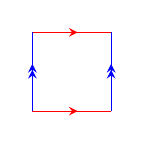
\begin{tikzpicture}
  \fill[white] (-.06,-.06) rectangle (1.06,1.06);
  \draw[-{stealth}, red] (0,0) -- (.575,0);
  \draw[red] (0,0) -- (1,0);
  \draw[-{stealth}, red] (0,1) -- (.575,1);
  \draw[red] (0,1) -- (1,1);
  \draw[-{stealth}, blue] (0,0) -- (0,.6);
  \draw[-{stealth}, blue] (0,0) -- (0,.525);
  \draw[blue] (0,0) -- (0,1);
  \draw[-{stealth}, blue] (1,0) -- (1,.6);
  \draw[-{stealth}, blue] (1,0) -- (1,.525);
  \draw[blue] (1,1) -- (1,0);
\end{tikzpicture}

%% Torus_3D (Homology-3.png)
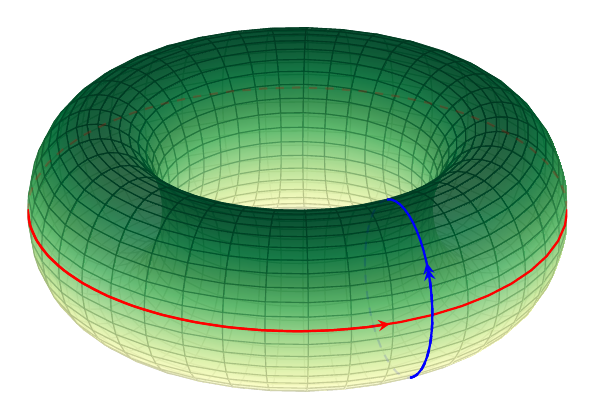
\begin{tikzpicture}
  \begin{axis}[view={180}{50}, axis lines=none, colormap/YlGn]
    % Draw the torus surface
    \addplot3[
      surf,
      shader=faceted interp, 
      samples=40,
      domain=0:360,
      y domain=0:360,
      z buffer=sort,
      opacity=.8
    ]
    (
      { (3 + cos(x)) * cos(y) },
      { (3 + cos(x)) * sin(y) },
      { sin(x) }
    );
    \addplot3+ [red, thick,
      domain=0:180,
        samples y=0,
        mark=none
    ]
    (
      { 4 * cos(x) },
      { 4 * sin(x) },
      { 0 }
    );
    \addplot3+ [red, thick,
      domain=0:110,
        samples y=0,
        mark=none,
        -{stealth}
    ]
    (
      { 4 * cos(x) },
      { 4 * sin(x) },
      { 0 }
    );
    \addplot3+ [red, thick, opacity=.2, dashed,
      domain=180:360,
        samples y=0,
        mark=none
    ]
    (
      { 4 * cos(x) },
      { 4 * sin(x) },
      { 0 }
    );
    \addplot3+ [blue, thick,
      domain=-70:110,
        samples y=0,
        mark=none
    ]
    (
      { (3 + cos(x)) * cos(120) },
      { (3 + cos(x)) * sin(120) },
      { sin(x) }
    );
    \addplot3+ [blue, thick,
      domain=-70:30,
        samples y=0,
        mark=none,
        -{stealth}
    ]
    (
      { (3 + cos(x)) * cos(120) },
      { (3 + cos(x)) * sin(120) },
      { sin(x) }
    );
    \addplot3+ [blue, thick,
      domain=-70:34,
        samples y=0,
        mark=none,
        -{stealth}
    ]
    (
      { (3 + cos(x)) * cos(120) },
      { (3 + cos(x)) * sin(120) },
      { sin(x) }
    );
    \addplot3+ [blue, thick, opacity=.1, dashed,
      domain=110:290,
        samples y=0,
        mark=none
    ]
    (
      { (3 + cos(x)) * cos(120) },
      { (3 + cos(x)) * sin(120) },
      { sin(x) }
    );
  \end{axis}
\end{tikzpicture}

%% Mobius_strip_2D (Homology-4.png)
\begin{tikzpicture}
  \fill[white] (-.06,-.06) rectangle (1.06,1.06);
  \draw[-{stealth}, red] (0,0) -- (.575,0);
  \draw[red] (0,0) -- (1,0);
  \draw[-{stealth}, red] (1,1) -- (.425,1);
  \draw[red] (0,1) -- (1,1);
  \draw[green!50!black] (0,0) -- (0,1);
  \draw[green!50!black] (1,1) -- (1,0);
\end{tikzpicture}

%% Mobius_strip_3D (Homology-5.png)
 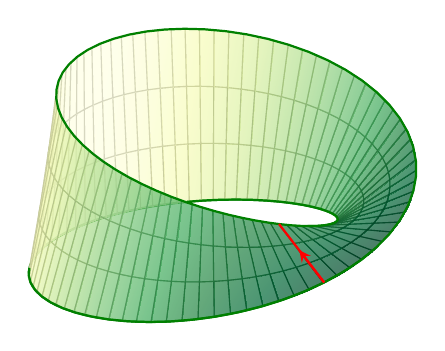
\begin{tikzpicture}
    \begin{axis}[
    hide axis,
    view = {40}{40},
    colormap/YlGn
    ]
    \addplot3 [color=green!50!black,thick,    
    domain     = 360:720,samples y=0, samples=80,
    ] (
    {(1+0.5*0.5*cos(x/2)))*cos(x)},
    {(1+0.5*0.5*cos(x/2)))*sin(x)},
    {0.5*0.5*sin(x/2)}
    );
    \addplot3 [
    surf,
    shader     = faceted interp,opacity = 0.7,
    %shader = interp,
    point meta = x,
    samples    = 80,
    samples y  = 4,
    z buffer   = sort,
    domain     = 0:360,
    y domain   =-0.5:0.5
    ] (
    {(1+0.5*y*cos(x/2)))*cos(x)},
    {(1+0.5*y*cos(x/2)))*sin(x)},
    {0.5*y*sin(x/2)}
    );
    \addplot3 [color=green!50!black,thick,    
    domain     = -140:497.5,samples y=0,samples=100,
    ] (
    {(1+0.5*0.5*cos(x/2)))*cos(x)},
    {(1+0.5*0.5*cos(x/2)))*sin(x)},
    {0.5*0.5*sin(x/2)}
    );
    \addplot3 [color=red,thick,    
    domain     = -.5:.5,samples y=0,samples=100,
    ] (
    {(1+0.5*x*cos(171)))*cos(342)},
    {(1+0.5*x*cos(171)))*sin(342)},
    {0.5*x*sin(171)}
    );
    \addplot3 [color=red,thick,    
    domain     = -.5:.05,samples y=0,samples=100,-{stealth}
    ] (
    {(1+0.5*x*cos(171)))*cos(342)},
    {(1+0.5*x*cos(171)))*sin(342)},
    {0.5*x*sin(171)}
    );
    \end{axis}
 \end{tikzpicture}

 %% Torus (Homology-6.png)
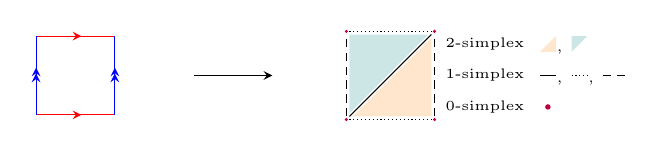
\begin{tikzpicture}
  \draw[white] (-.1,-.1) rectangle (7.5,1.1);
  \draw[-{stealth}, red] (0,0) -- (.575,0);
  \draw[red] (0,0) -- (1,0);
  \draw[-{stealth}, red] (0,1) -- (.575,1);
  \draw[red] (0,1) -- (1,1);
  \draw[-{stealth}, blue] (0,0) -- (0,.6);
  \draw[-{stealth}, blue] (0,0) -- (0,.525);
  \draw[blue] (0,0) -- (0,1);
  \draw[-{stealth}, blue] (1,0) -- (1,.6);
  \draw[-{stealth}, blue] (1,0) -- (1,.525);
  \draw[blue] (1,1) -- (1,0);

  \draw[-{stealth}] (2,.5) -- (3,.5);
  \fill[orange, opacity=.2] (4.02,-.02) -- (5.02,-.02) -- (5.02,0.98) -- cycle;
  \fill[teal, opacity=.2] (3.98,0.02) -- (3.98,1.02) -- (4.98,1.02) -- cycle;
  \draw (3.98,-.02) -- (5.02,1.02);
  \draw[densely dashed] (3.94,-.02) -- (3.94,1.02);
  \draw[densely dotted] (3.98,1.06) -- (5.02,1.06);
  \draw[densely dashed] (5.06,-.02) -- (5.06,1.02);
  \draw[densely dotted] (3.98,-.06) -- (5.02,-.06);
  \fill[purple] (3.94,1.06) circle[radius=.6pt];
  \fill[purple] (5.06,1.06) circle[radius=.6pt];
  \fill[purple] (3.94,-.06) circle[radius=.6pt];
  \fill[purple] (5.06,-.06) circle[radius=.6pt];
  \draw (5.7,.9) node{\tiny $2$-simplex};
  \fill[orange, opacity=.2] (6.4,.8)--(6.6,.8)--(6.6,1)--cycle;
  \draw (6.65,.8) node{\tiny,};
  \fill[teal, opacity=.2] (6.8,.8)--(6.8,1)--(7,1)--cycle;
  \draw (5.7,.5) node{\tiny $1$-simplex};
  \draw (6.4,.5)--(6.6,.5);
  \draw (6.65,.4) node{\tiny,};
  \draw[densely dotted] (6.8,.5)--(7,.5);
  \draw (7.05,.4) node{\tiny,};
  \draw[densely dashed] (7.2,.5)--(7.5,.5);
  \draw (5.7,.1) node{\tiny $0$-simplex};
  \fill[purple] (6.5,.1) circle[radius=1pt];
\end{tikzpicture}

%%Finer_torus (Homology-7.png)
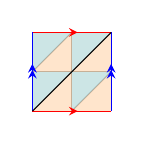
\begin{tikzpicture}
  \fill[white] (-.06,-.06) rectangle (1.06,1.06);
  \draw[gray!50] (.5,0)--(.5,1);
  \draw[gray!50] (0,.5)--(1,.5);
  \draw[gray!50] (0,.5)--(.5,1);
  \draw[gray!50] (.5,0)--(1,.5);
  \fill[teal, opacity=.2] (0,0) -- (.5,.5) -- (0,.5) -- cycle;
  \fill[teal, opacity=.2] (0,.5) -- (.5,1) -- (0,1) -- cycle;
  \fill[teal, opacity=.2] (.5,.5) -- (1,1) -- (.5,1) -- cycle;
  \fill[teal, opacity=.2] (.5,0) -- (1,.5) -- (.5,.5) -- cycle;
  \fill[orange, opacity=.2] (0,0) -- (.5,.5) -- (.5,0) -- cycle;
  \fill[orange, opacity=.2] (0,.5) -- (.5,1) -- (.5,.5) -- cycle;
  \fill[orange, opacity=.2] (.5,.5) -- (1,1) -- (1,.5) -- cycle;
  \fill[orange, opacity=.2] (.5,0) --(1,.5) -- (1,0) -- cycle;
  \draw[-{stealth}, red] (0,0) -- (.575,0);
  \draw[red] (0,0) -- (1,0);
  \draw[-{stealth}, red] (0,1) -- (.575,1);
  \draw[red] (0,1) -- (1,1);
  \draw[-{stealth}, blue] (0,0) -- (0,.6);
  \draw[-{stealth}, blue] (0,0) -- (0,.525);
  \draw[blue] (0,0) -- (0,1);
  \draw[-{stealth}, blue] (1,0) -- (1,.6);
  \draw[-{stealth}, blue] (1,0) -- (1,.525);
  \draw[blue] (1,1) -- (1,0);
  \draw (0,0) -- (1,1);
\end{tikzpicture}

%% Torus_upper (Homology-8.png)
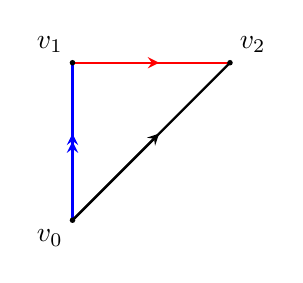
\begin{tikzpicture}[scale=2]
  \draw[-{stealth}, blue, thick] (0,0)--(0,.55); 
  \draw[-{stealth}, blue, thick] (0,0)--(0,.5);
  \draw[blue, thick] (0,0)--(0,1);
  \draw[red, thick] (0,1)--(1,1);
  \draw[red, thick, -{stealth}] (0,1)--(.55,1);
  \draw[thick] (0,0)--(1,1);
  \draw[thick,-{stealth}] (0,0)--(.55,.55);
  \fill (0,0) circle[radius=.5pt] node[below left]{$v_0$};
  \fill (0,1) circle[radius=.5pt] node[above left]{$v_1$};
  \fill (1,1) circle[radius=.5pt] node[above right]{$v_2$};
\end{tikzpicture}

%% Torus_lower (Homology-9.png)
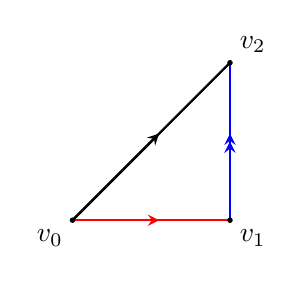
\begin{tikzpicture}[scale=2]
  \draw[-{stealth}, blue, thick] (1,0)--(1,.55); 
  \draw[-{stealth}, blue, thick] (1,0)--(1,.5);
  \draw[blue, thick] (1,0)--(1,1);
  \draw[red, thick] (0,0)--(1,0);
  \draw[red, thick, -{stealth}] (0,0)--(.55,0);
  \draw[thick] (0,0)--(1,1);
  \draw[thick,-{stealth}] (0,0)--(.55,.55);
  \fill (0,0) circle[radius=.5pt] node[below left]{$v_0$};
  \fill (1,0) circle[radius=.5pt] node[below right]{$v_1$};
  \fill (1,1) circle[radius=.5pt] node[above right]{$v_2$};
\end{tikzpicture}

%% cycle_in_D2 (Homology-10.png)
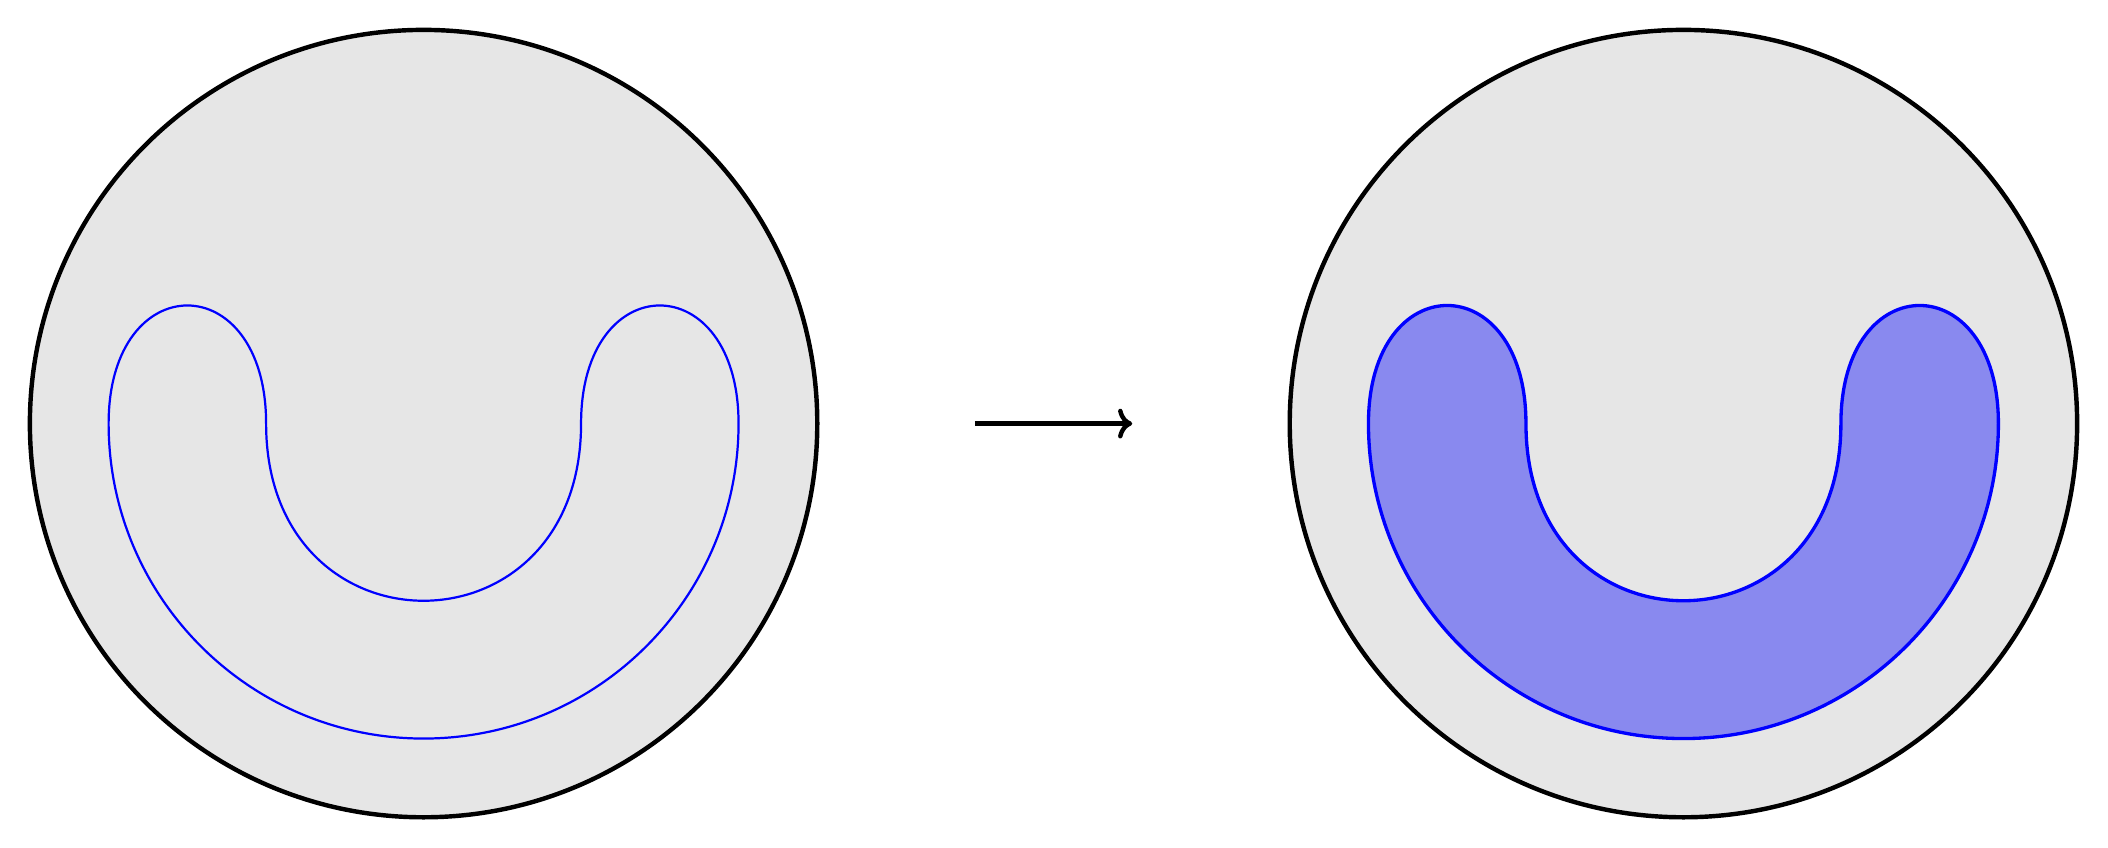
\begin{tikzpicture}
  \filldraw[fill=gray, fill opacity=.2, draw=black, ultra thick] (0,0) circle[radius=5];
  \draw[blue, thick] (4,0) arc (0:-180:4) .. controls (-4,2) and (-2,2) .. (-2,0) ..controls (-2,-3) and (2,-3) .. (2,0) .. controls (2,2) and (4,2) .. (4,0);
  \draw[->, ultra thick] (7,0)--(9,0);
  \begin{scope}[shift={(16,0)}]
    \filldraw[fill=gray, fill opacity=.2, draw=black, ultra thick] (0,0) circle[radius=5];
    \filldraw[fill=blue, fill opacity=.4, draw=blue, very thick] (4,0) arc (0:-180:4) .. controls (-4,2) and (-2,2) .. (-2,0) ..controls (-2,-3) and (2,-3) .. (2,0) .. controls (2,2) and (4,2) .. (4,0);
  \end{scope}
\end{tikzpicture}

%% cycle_in_punctured_D2 (Homology-11.png)
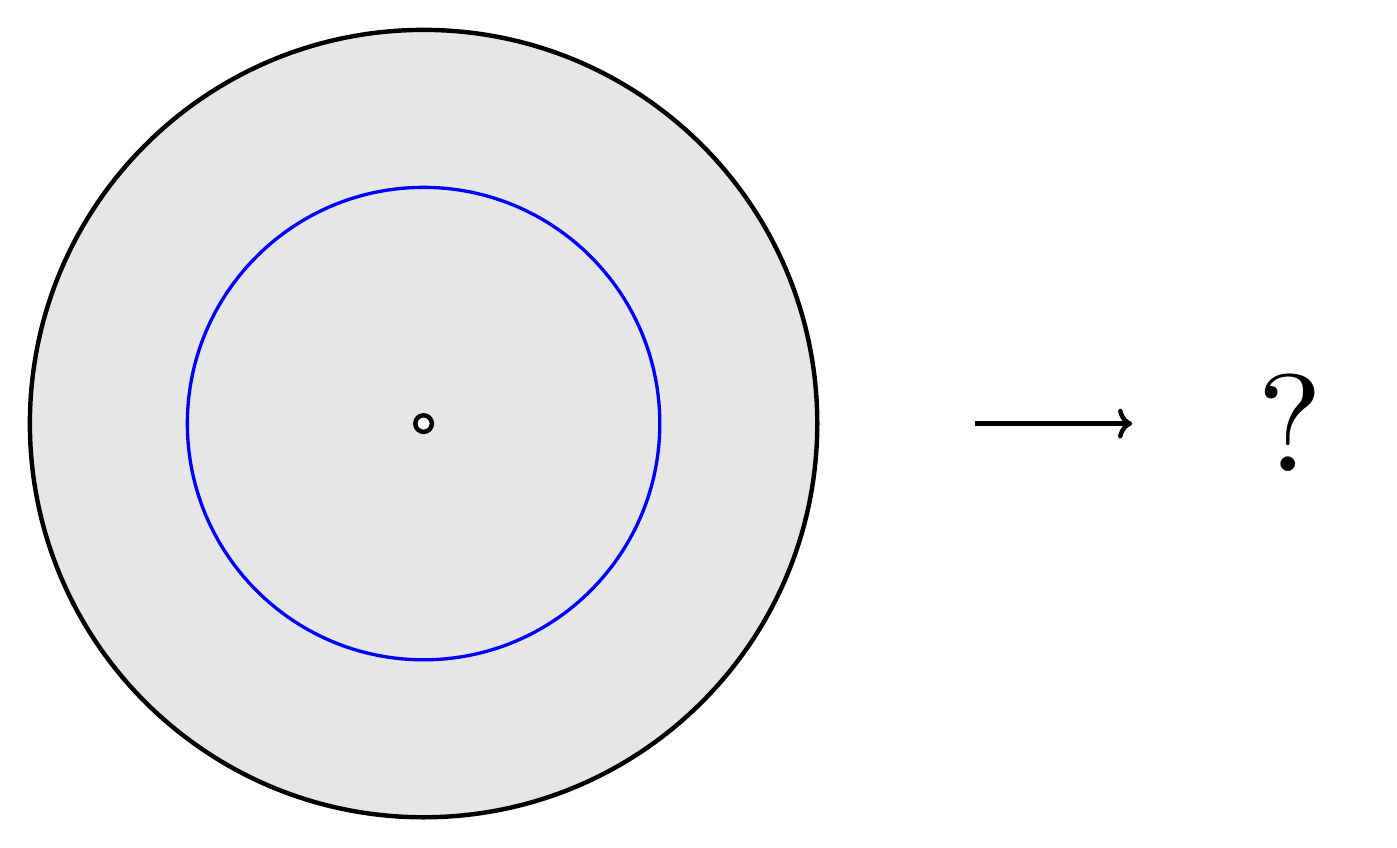
\begin{tikzpicture}
  \filldraw[fill=gray, fill opacity=.2, draw=black, ultra thick] (0,0) circle[radius=5];
  \filldraw[fill=white, draw=black, ultra thick] (0,0) circle[radius=3pt];
  \draw[blue, very thick] (0,0) circle[radius=3];
  \draw[->, ultra thick] (7,0)--(9,0);
  \draw (11,0) node[scale=5] {?};
\end{tikzpicture}

%% cycle_in_punctured_D3 (Homology-12.png)
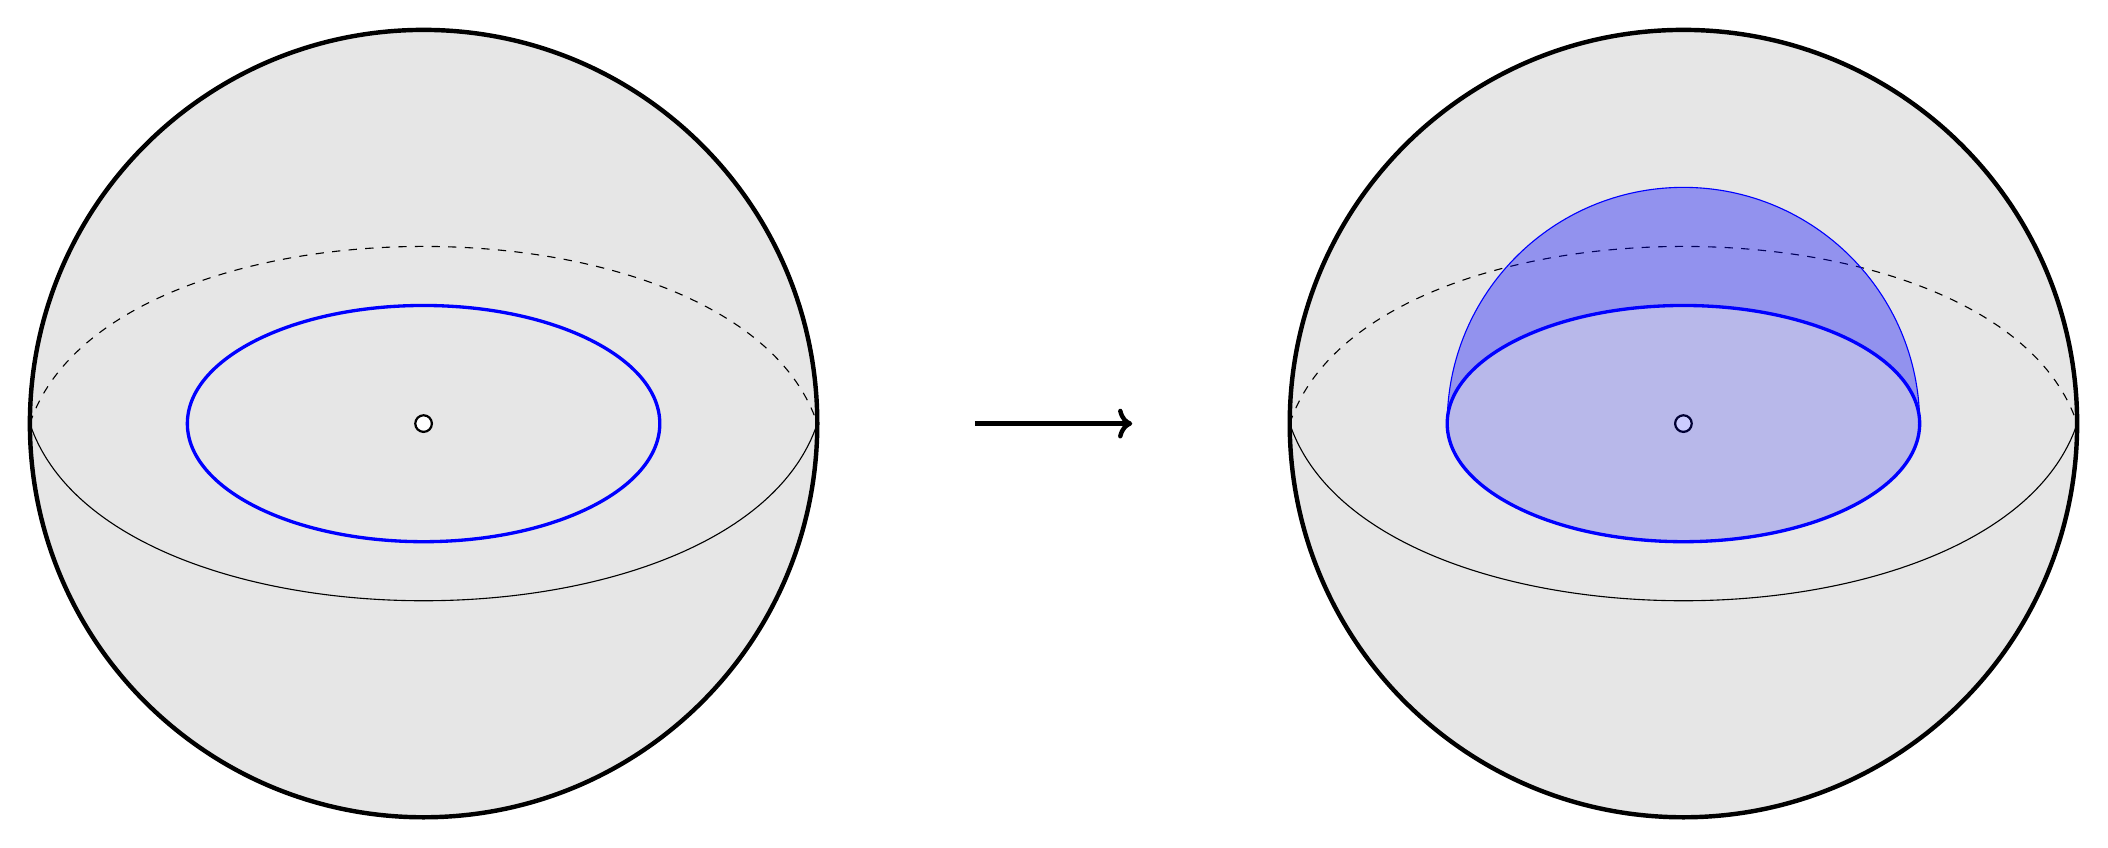
\begin{tikzpicture}
  \filldraw[fill=gray, fill opacity=.2, draw=black, ultra thick] (0,0) circle[radius=5];
  \draw (-5,0) .. controls (-4,-3) and (4,-3) .. (5,0);
  \draw[dashed] (-5,0) .. controls (-4,3) and (4,3) .. (5,0);
  \filldraw[fill=white, draw=black, thick] (0,0) circle[radius=3pt];
  \draw[blue, very thick] (0,0) ellipse (3cm and 1.5cm);
  \draw[->, ultra thick] (7,0)--(9,0);
  \begin{scope}[shift={(16,0)}]
    \filldraw[fill=gray, fill opacity=.2, draw=black, ultra thick] (0,0) circle[radius=5];
    \draw (-5,0) .. controls (-4,-3) and (4,-3) .. (5,0);
    \draw[dashed] (-5,0) .. controls (-4,3) and (4,3) .. (5,0);
    \filldraw[fill=white, draw=black, thick] (0,0) circle[radius=3pt];
    \fill[blue, opacity=.2] (3,0) arc (0:180:3cm) arc (180:360:3cm and 1.5cm);
    \fill[blue, opacity=.2] (3,0) arc (0:180:3cm) arc (180:0:3cm and 1.5cm);
    \draw[blue, very thick] (0,0) ellipse (3cm and 1.5cm);
    \draw[blue] (3,0) arc (0:180:3cm);
  \end{scope}
\end{tikzpicture}



%% Prism (Homotopy-1.png)
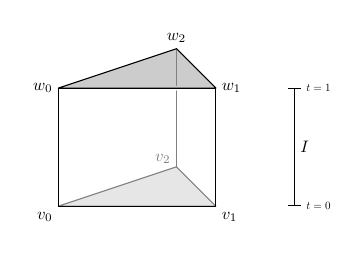
\begin{tikzpicture}[line join=round, line cap=round]
  \fill[draw=gray, fill=gray, fill opacity=.2] (0,0) -- (2,0) -- (1.5,.5) -- cycle; 
  \path[name path=1] (1.5,.5) -- (1.5,2);
  \path[name path=2] (1.5,2) -- (0,0);
  \path[name path=3] (1.5,2) -- (2,0);
  \path[name path=4] (0,1.5) -- (2,1.5);
  \path[name intersections={of=1 and 4, by=14}];
  \draw[gray, shorten >=1pt] (1.5,.5) -- (14);
  \draw[gray, shorten <=1pt] (14) -- (1.5,2);
  \draw (0,0) -- (2,0) -- (2,1.5) -- (0,1.5) -- cycle;
  \filldraw[fill=gray, fill opacity=.4] (0,1.5) -- (2,1.5) -- (1.5,2) -- cycle;
  \draw (0,0) node[below left, scale=.6]{$v_0$};
  \draw (2,0) node[below right, scale=.6]{$v_1$};
  \draw (1.5,.6) node[left, scale=.6, gray]{$v_2$};
  \draw (0,1.5) node[left, scale=.6]{$w_0$};
  \draw (2,1.5) node[right, scale=.6]{$w_1$};
  \draw (1.5,2) node[above, scale=.6]{$w_2$};
  \draw[|-|] (3,0) -- (3,1.5);
  \draw (3,.75) node[right, scale=.6]{$I$};
  \draw (3.1,0) node[right, scale=.4]{$t=0$};
  \draw (3.1,1.5) node[right, scale=.4]{$t=1$};
\end{tikzpicture}

%% Prism_sliced (Homotopy-2.png)
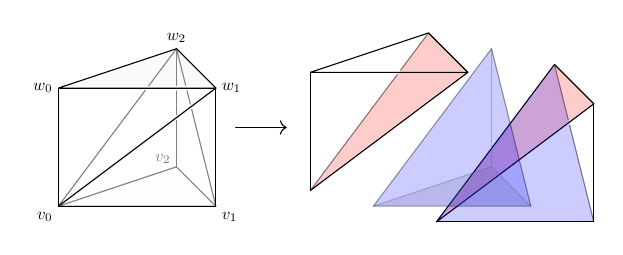
\begin{tikzpicture}[line join=round, line cap=round]
    \begin{scope}[shift={(-4,0)}]
      \fill[draw=gray, fill=gray, fill opacity=.02] (0,0) -- (2,0) -- (1.5,.5) -- cycle; 
      \path[name path=1] (1.5,.5) -- (1.5,2);
      \path[name path=2] (1.5,2) -- (0,0);
      \path[name path=3] (1.5,2) -- (2,0);
      \path[name path=4] (0,1.5) -- (2,1.5);
      \path[name path=5] (0,0) -- (2,1.5);
      \path[name intersections={of=1 and 4, by=14}];
      \path[name intersections={of=1 and 5, by=15}];
      \path[name intersections={of=2 and 4, by=24}];
      \path[name intersections={of=3 and 4, by=34}];
      \path[name intersections={of=3 and 5, by=35}];
      \draw[gray, shorten >=1pt] (1.5,.5) -- (15);
      \draw[gray, shorten <=1pt, shorten >=1pt] (15) -- (14);
      \draw[gray, shorten <=1pt] (14) -- (1.5,2);
      \draw[gray, shorten >=1pt] (0,0) -- (24);
      \draw[gray, shorten <=1pt] (24) -- (1.5,2);
      \draw[gray, shorten >=1pt] (1.5,2) -- (34);
      \draw[gray, shorten <=1pt, shorten >=1pt] (34) -- (35);
      \draw[gray, shorten <=1pt] (35) -- (2,0);
      \draw (0,0) -- (2,0) -- (2,1.5) -- (0,1.5) -- cycle;
      \draw (0,0) -- (2,1.5);
      \filldraw[fill=gray, fill opacity=.04] (0,1.5) -- (2,1.5) -- (1.5,2) -- cycle;
      \draw (0,0) node[below left, scale=.6]{$v_0$};
      \draw (2,0) node[below right, scale=.6]{$v_1$};
      \draw (1.5,.6) node[left, scale=.6, gray]{$v_2$};
      \draw (0,1.5) node[left, scale=.6]{$w_0$};
      \draw (2,1.5) node[right, scale=.6]{$w_1$};
      \draw (1.5,2) node[above, scale=.6]{$w_2$};
    \end{scope}
    \draw[->] (-1.75,1) -- (-1.1,1);
    \begin{scope}[shift={(-.8,.2)}]
      \path[name path=1] (1.5,.5) -- (1.5,2);
      \path[name path=2] (1.5,2) -- (0,0);
      \path[name path=3] (1.5,2) -- (2,0);
      \path[name path=4] (0,1.5) -- (2,1.5);
      \path[name path=5] (0,0) -- (2,1.5);
      \path[name intersections={of=1 and 4, by=14}];
      \path[name intersections={of=1 and 5, by=15}];
      \path[name intersections={of=2 and 4, by=24}];
      \path[name intersections={of=3 and 4, by=34}];
      \path[name intersections={of=3 and 5, by=35}];
      \draw[gray, shorten >=1pt] (0,0) -- (24);
      \draw[gray, shorten <=1pt] (24) -- (1.5,2);
      \fill[red, opacity=.2] (0,0) -- (1.5,2) -- (2,1.5) -- cycle;
      \draw (0,0) -- (0,1.5);
      \draw (0,0) -- (2,1.5);
      \draw (0,1.5) -- (2,1.5) -- (1.5,2) -- cycle;
    \end{scope}
    \begin{scope}[shift={(.8,-.2)}]
      \path[name path=1] (1.5,.5) -- (1.5,2);
      \path[name path=2] (1.5,2) -- (0,0);
      \path[name path=3] (1.5,2) -- (2,0);
      \path[name path=4] (0,1.5) -- (2,1.5);
      \path[name path=5] (0,0) -- (2,1.5);
      \path[name intersections={of=1 and 4, by=14}];
      \path[name intersections={of=1 and 5, by=15}];
      \path[name intersections={of=2 and 4, by=24}];
      \path[name intersections={of=3 and 4, by=34}];
      \path[name intersections={of=3 and 5, by=35}];
      \draw[gray, shorten >=1pt] (1.5,2) -- (35);
      \draw[gray, shorten <=1pt] (35) -- (2,0);
      \filldraw[fill=red, fill opacity=.2] (0,0) -- (1.5,2) -- (2,1.5) -- cycle;
      \fill[blue, opacity=.2] (0,0) -- (1.5,2) -- (2,0) --cycle;
      \draw (0,0) -- (2,0) -- (2,1.5);
    \end{scope}
    \begin{scope}[opacity=.4]
    \draw[gray] (2,0)-- (1.5,.5) -- (0,0); 
    \draw[gray] (1.5,2)--(1.5,.5);
    \draw (0,0) -- (1.5,2) -- (2,0) -- cycle;
    \fill[gray, opacity=.2] (0,0) -- (2,0) -- (1.5,.5) -- cycle; 
    \fill[blue, opacity=.2] (1.5,2) -- (2,0) -- (0,0) --cycle;
    \end{scope}
\end{tikzpicture}

%% homotopy_invariance_of_Pi (Homotopy-3.png)
\begin{tikzcd}
  f_0(x_0) \rar["{[f_0\circ\alpha]}"]\dar["f_t(x_0)" left]&[20pt]f_0(x_1)\dar["f_t(x_1)"]\\
  f_1(x_0) \rar["{[f_1\circ\alpha]}" below]&f_1(x_1)
\end{tikzcd}


%% Covering_space (Covering_spaces-1.png)
\begin{tikzpicture}
   \begin{axis}[
 view={-20}{-20},
 zmax=80,
  xmax=2,
   ymax=2,
 height=12cm,
 clip=false,hide axis
]
\addplot3+[domain=0:2.5,samples=500,samples y=0,black,no marks,thick] 
({sin(deg(x))}, 
{cos(deg(x))}, 
{2+4*x});
\addplot3+[domain=2.6:2.5+2*pi,samples=500,samples y=0,black,no marks,thick] 
({sin(deg(x))}, 
{cos(deg(x))}, 
{2+4*x});
\addplot3+[domain=2.6+2*pi:2.5+4*pi,samples=500,samples y=0,black,no marks,thick] 
({sin(deg(x))}, 
{cos(deg(x))}, 
{2+4*x});
\addplot3+[domain=2.6+4*pi:8*pi,samples=500,samples y=0,black,no marks,thick] 
({sin(deg(x))}, 
{cos(deg(x))}, 
{2+4*x});
\addplot3+[domain=0:2*pi,samples=500,samples y=0,black,no marks,very thick] 
({sin(deg(x))}, 
{cos(deg(x))}, 
-50);
\addplot3+[domain=0.5:1,samples=3000,samples y=0,orange,no marks,ultra thick,{Parenthesis}-{Parenthesis}] 
({sin(deg(x))}, 
{cos(deg(x))}, 
-50);
\addplot3+[domain=0.5:1,samples=3000,samples y=0,orange,no marks,very thick,{Parenthesis}-{Parenthesis}] 
({sin(deg(x))}, 
{cos(deg(x))}, 
{2+4*x});
\addplot3+[domain=0.5+2*pi:1+2*pi,samples=3000,samples y=0,orange,no marks,very thick,{Parenthesis}-{Parenthesis}] 
({sin(deg(x))}, 
{cos(deg(x))}, 
{2+4*x});
\addplot3+[domain=0.5+4*pi:1+4*pi,samples=3000,samples y=0,orange,no marks,very thick,{Parenthesis}-{Parenthesis}] 
({sin(deg(x))}, 
{cos(deg(x))}, 
{2+4*x});
\addplot3+[domain=0.5+6*pi:1+6*pi,samples=3000,samples y=0,orange,no marks,very thick,{Parenthesis}-{Parenthesis}] 
({sin(deg(x))}, 
{cos(deg(x))}, 
{2+4*x});
\end{axis}
\draw (10,5.5) node{$E$};
\draw (10,3) node{$B$};
\draw[->] (10,5) -- (10,3.5) node[midway, right]{$p$};
\end{tikzpicture}

%% morphism_of_covering_spaces (Covering_spaces-2.png)
\begin{tikzcd}
  E\arrow[rr]\drar&[-15pt]&[-15pt]E'\dlar\\
  &B
\end{tikzcd}

%% colimit_in_Top (Covering_spaces-3.png)
\begin{tikzcd}
  U\rar[hook]&X\\
  U\cap V\uar[hook]\rar[hook]&V\uar[hook]
\end{tikzcd}

%% colimit_in_Top_generalized (Covering_spaces-4.png)
\begin{tikzcd}
  U_i\rar[hook]&X\\
  U_i\cap U_j\uar[hook]\rar[hook]&U_j\uar[hook]
\end{tikzcd}

%% classical_van_Kampen (Covering_spaces-5.png)
\begin{tikzcd}
  {\pi_1(U)} & {\pi_1(U)\ast_{\pi_1(U\cap V)}\pi_1(V)} \\
  {\pi_1(U\cap V)} & {\pi_1(V)}
  \arrow[from=1-1, to=1-2]
  \arrow[from=2-1, to=1-1]
  \arrow[from=2-1, to=2-2]
  \arrow[from=2-2, to=1-2]
\end{tikzcd}

%% realtive_homology (Computation_of_homology-1.png)
\begin{tikzcd}
  C_\bullet(A)\rar[hook]\dar["C_\bullet(f\vert_A)" left]&C_\bullet(X)\dar["C_\bullet(f)"]\\
  C_\bullet(B)\rar[hook]&C_\bullet(Y)
\end{tikzcd}

%% double_relative (Computation_of_homology-2.png)
\begin{tikzcd}
  & 0 & 0 & 0 \\
  0 & {C_\bullet(A)} & {C_\bullet(U)} & {C_\bullet(U,A)} & 0 \\
  0 & {C_\bullet(A)} & {C_\bullet(X)} & {C_\bullet(X,A)} & 0 \\
  0 & 0 & {C_\bullet(X,U)} & {C_\bullet(X,U)} & 0 \\
  & 0 & 0 & 0
  \arrow[from=1-2, to=2-2]
  \arrow[from=1-3, to=2-3]
  \arrow[from=1-4, to=2-4]
  \arrow[from=2-1, to=2-2]
  \arrow[from=2-2, to=2-3]
  \arrow[equals, from=2-2, to=3-2]
  \arrow[from=2-3, to=2-4]
  \arrow[from=2-3, to=3-3]
  \arrow[from=2-4, to=2-5]
  \arrow[from=2-4, to=3-4]
  \arrow[from=3-1, to=3-2]
  \arrow[from=3-2, to=3-3]
  \arrow[from=3-2, to=4-2]
  \arrow[from=3-3, to=3-4]
  \arrow[from=3-3, to=4-3]
  \arrow[from=3-4, to=3-5]
  \arrow[from=3-4, to=4-4]
  \arrow[from=4-1, to=4-2]
  \arrow[from=4-2, to=4-3]
  \arrow[from=4-2, to=5-2]
  \arrow[equals, from=4-3, to=4-4]
  \arrow[from=4-3, to=5-3]
  \arrow[from=4-4, to=4-5]
  \arrow[from=4-4, to=5-4]
\end{tikzcd}
  
%% excision_1 (Compuatation_of_homology-3.png)
\begin{tikzcd}
  H_k(X,A)\rar\dar&H_k(X,U)\dar\\
  H_k(X/A,[A])\rar&H_k(X/A,U/A)
\end{tikzcd}

%% excision_2 (Computation_of_homology-4.png)
\begin{tikzcd}
  H_k(X\setminus A, U\setminus A)\rar\dar&H_k(X,U)\dar\\
  H_k((X/A)\setminus[A], (U/A)\setminus[A])\rar& H_k(X/A,U/A)
\end{tikzcd}

%% functoriality (Computation_of_homology-5.png)
\begin{tikzcd}
  \cdots & {H_k(A)} & {H_k(X)} & {H_k(X,A)} & {H_{k-1}(A)} & \cdots \\
  \cdots & {H_k(A)} & {H_k(X)} & {H_k(X/A)} & {H_{k-1}(A)} & \cdots
  \arrow[from=1-1, to=1-2]
  \arrow[from=1-2, to=1-3]
  \arrow[equals, from=1-2, to=2-2]
  \arrow[from=1-3, to=1-4]
  \arrow[equals, from=1-3, to=2-3]
  \arrow[from=1-4, to=1-5]
  \arrow[from=1-4, to=2-4]
  \arrow[from=1-5, to=1-6]
  \arrow[equals, from=1-5, to=2-5]
  \arrow[from=2-1, to=2-2]
  \arrow[from=2-2, to=2-3]
  \arrow[from=2-3, to=2-4]
  \arrow[from=2-4, to=2-5]
  \arrow[from=2-5, to=2-6]
\end{tikzcd}

%% induction (Computation_of_homology-6.png)
\begin{tikzcd}
  \cdots & {H^\Delta_n(X^k,X^{k-1})} & {H^\Delta_{n-1}(X^{k-1})} & {H^\Delta_{n-1}(X^k)} & {H_{n-1}^\Delta(X^k,X^{k-1})} & {H^\Delta_{n-2}(X^{k-1})} & \cdots \\
  \cdots & {H_n(X^k,X^{k-1})} & {H_{n-1}(X^{k-1})} & {H_{n-1}(X^k)} & {H_{n-1}(X^k,X^{k-1})} & {H_{n-2}(X^{k-1})} & \cdots
  \arrow[from=1-1, to=1-2]
  \arrow[from=1-2, to=1-3]
  \arrow[from=1-2, to=2-2]
  \arrow[from=1-3, to=1-4]
  \arrow[from=1-3, to=2-3]
  \arrow[from=1-4, to=1-5]
  \arrow[from=1-4, to=2-4]
  \arrow[from=1-5, to=1-6]
  \arrow[from=1-5, to=2-5]
  \arrow[from=1-6, to=1-7]
  \arrow[from=1-6, to=2-6]
  \arrow[from=2-1, to=2-2]
  \arrow[from=2-2, to=2-3]
  \arrow[from=2-3, to=2-4]
  \arrow[from=2-4, to=2-5]
  \arrow[from=2-5, to=2-6]
  \arrow[from=2-6, to=2-7]
\end{tikzcd}

%% inclusions (Computation_of_homology-7.png)
\begin{tikzcd}
  U\rar[hook]&X\\
  U\cap V \uar[hook]\rar[hook]&V\uar[hook]
\end{tikzcd}

%% morphism_of_les (Computation_of_homology-8.png)
\begin{tikzcd}
  \cdots & {H_{n+1}(V, U\cap V)} & {H_n(U\cap V)} & {H_n(V)} & {H_n(V,U\cap V)} & \cdots \\
  \cdots & {H_{n+1}(X,U)} & {H_n(U)} & {H_n(X)} & {H_n(X,U)} & \cdots
  \arrow["p_V", from=1-1, to=1-2]
  \arrow["\partial_V", from=1-2, to=1-3]
  \arrow["i_V", from=1-2, to=2-2]
  \arrow["j_V", from=1-3, to=1-4]
  \arrow["j_U", from=1-3, to=2-3]
  \arrow["p_V", from=1-4, to=1-5]
  \arrow["k_V", from=1-4, to=2-4]
  \arrow["\partial_V", from=1-5, to=1-6]
  \arrow["i_V", from=1-5, to=2-5]
  \arrow["p_X", from=2-1, to=2-2]
  \arrow["\partial_X", from=2-2, to=2-3]
  \arrow["k_U", from=2-3, to=2-4]
  \arrow["p_X", from=2-4, to=2-5]
  \arrow["\partial_X", from=2-5, to=2-6]
\end{tikzcd}

%% Proof_of_UCT (Cohomology-1.png)
\begin{tikzcd}
  0 & {Z_n\otimes_\mathbb{Z}A} & {C_n\otimes_\mathbb{Z}A} & {B_{n-1}\otimes_\mathbb{Z}A} & 0 \\
  0 & {Z_{n-1}\otimes_\mathbb{Z}A} & {C_{n-1}\otimes_\mathbb{Z}A} & {B_{n-2}\otimes_\mathbb{Z}A} & 0
  \arrow[from=1-1, to=1-2]
  \arrow["{\iota_n\otimes \id_A}", from=1-2, to=1-3]
  \arrow["0", from=1-2, to=2-2]
  \arrow["{\partial_n\otimes \id_A}", from=1-3, to=1-4]
  \arrow["{\partial_n\otimes \id_A}", from=1-3, to=2-3]
  \arrow[from=1-4, to=1-5]
  \arrow["0", from=1-4, to=2-4]
  \arrow[from=2-1, to=2-2]
  \arrow["{\iota_{n-1}\otimes\id_A}"', from=2-2, to=2-3]
  \arrow["{\partial_{n-1}\otimes\id_A}"', from=2-3, to=2-4]
  \arrow[from=2-4, to=2-5]
\end{tikzcd}


%% lifting (Acyclic_models_theorem-1.png)
\begin{tikzcd}
  {F_0(X)} & {G_0(X)} \\
  {H_0(F(X))} & {H_0(G(X))}
  \arrow["{f_0(X)}", dashed, from=1-1, to=1-2]
  \arrow["{p_F}"', from=1-1, to=2-1]
  \arrow[from=1-1, to=2-2]
  \arrow["{p_G}"', from=1-2, to=2-2]
  \arrow["{f(X)_0}"', from=2-1, to=2-2]
\end{tikzcd}

%% lifting_general (Acyclic_models_theorem-2.png)
\begin{tikzcd}
  {F_n(X)} & {F_{n-1}(X)} & {F_{n-2}(X)} & \cdots \\
  {G_n(X)} & {G_{n-1}(X)} & {G_{n-2}(X)} & \cdots
  \arrow["{d_n^{F(X)}}", from=1-1, to=1-2]
  \arrow[dashed, from=1-1, to=2-1]
  \arrow["{d_{n-1}^{F(X)}}", from=1-2, to=1-3]
  \arrow["{f_{n-1}(X)}"', from=1-2, to=2-2]
  \arrow[from=1-3, to=1-4]
  \arrow["{f_{n-2}(X)}"', from=1-3, to=2-3]
  \arrow["{d_n^{G(X)}}"', from=2-1, to=2-2]
  \arrow["{d_{n-1}^{G(X)}}"', from=2-2, to=2-3]
  \arrow[from=2-3, to=2-4]
\end{tikzcd}

%% reduction_to_models (Acyclic_models_theorem-3.png)
\begin{tikzcd}
  {F_n(M)} & {F_n(X)} \\
  {G_n(M)} & {G_n(X)}
  \arrow["{F_n(u)}", from=1-1, to=1-2]
  \arrow["{f_n(M)}"', from=1-1, to=2-1]
  \arrow["{G_n(u)}"', from=2-1, to=2-2]
\end{tikzcd}

%% lifting_reduced (Acyclic_models_theorem-4.png)
\begin{tikzcd}
  {F_n(M)} & {F_{n-1}(M)} & {F_{n-2}(M)} & \cdots \\
  {G_n(M)} & {G_{n-1}(M)} & {G_{n-2}(M)} & \cdots
  \arrow["{d_n^{F(M)}}", from=1-1, to=1-2]
  \arrow[dashed, from=1-1, to=2-1]
  \arrow["{d_{n-1}^{F(M)}}", from=1-2, to=1-3]
  \arrow["{f_{n-1}(M)}"', from=1-2, to=2-2]
  \arrow[from=1-3, to=1-4]
  \arrow["{f_{n-2}(M)}"', from=1-3, to=2-3]
  \arrow["{d_n^{G(M)}}"', from=2-1, to=2-2]
  \arrow["{d_{n-1}^{G(M)}}"', from=2-2, to=2-3]
  \arrow[from=2-3, to=2-4]
\end{tikzcd}

%% fliipping (Acyclic_models_theorem-5.png)
\begin{tikzcd}
  {C_\bullet(X;A)\otimes C_\bullet(Y;A)} & {C_\bullet(Y;A)\otimes C_\bullet (X;A)} \\
  {C_\bullet(X\times Y;A)} & {C_\bullet(Y\times X;A)}
  \arrow[from=1-1, to=1-2]
  \arrow[from=1-1, to=2-1]
  \arrow[from=1-2, to=2-2]
  \arrow[from=2-1, to=2-2]
\end{tikzcd}


%% functoriality_of_cross_product (Cup_products-1.png)
\begin{tikzcd}
  {H^\ast(X;A)\otimes H^\ast(Y;A)\otimes H^\ast(X;A)\otimes H^\ast(Y;A)} & {H^\ast(X\times Y;A)\otimes H^\ast(X\times Y;A)} \\
  {H^\ast(X;A)\otimes H^\ast(Y;A)} & {H^\ast(X\times Y;A)}
  \arrow["{\times\otimes\times}", from=1-1, to=1-2]
  \arrow["{\smile\otimes\smile}"', from=1-1, to=2-1]
  \arrow["\smile", from=1-2, to=2-2]
  \arrow["\times"', from=2-1, to=2-2]
\end{tikzcd}

%% functoriality (Cup_products-2.png)
\begin{tikzcd}
  {H^\bullet(Y;A)\otimes H^\bullet(Y;A)} & {H^\bullet(Y\times Y;A)} \\
  {H^\bullet(X;A)\otimes H^\bullet(X;A)} & {H^\bullet(X\times X;A)}
  \arrow[from=1-1, to=1-2]
  \arrow[from=1-1, to=2-1]
  \arrow[from=1-2, to=2-2]
  \arrow[from=2-1, to=2-2]
\end{tikzcd}

%% diagonal_and_f (Cup_products-3.png)
\begin{tikzcd}
  X & {X\times X} \\
  Y & {Y\times Y}
  \arrow["{\Delta_X}", from=1-1, to=1-2]
  \arrow["f"', from=1-1, to=2-1]
  \arrow["{(f,f)}", from=1-2, to=2-2]
  \arrow["{\Delta_Y}"', from=2-1, to=2-2]
\end{tikzcd}


%% Orientation_cover_of_S^1 (Poincare_duality-1.png)
\begin{tikzpicture}
   \begin{axis}[
 view={-20}{-20},
 zmax=80,
  xmax=2,
   ymax=2,
 height=12cm,
 clip=false,hide axis
]
\addplot3+[domain=0.7:1,samples=3000,samples y=0,red,no marks,thick,{stealth}-] 
({sin(deg(1.3))*x}, 
{cos(deg(1.3))*x}, 
-50);
\addplot3+[domain=1:1.3,samples=3000,samples y=0,blue,no marks,thick,-{stealth}] 
({sin(deg(1.3))*x}, 
{cos(deg(1.3))*x}, 
-50);
\addplot3+[domain=0:2*pi,samples=500,samples y=0,black,no marks,very thick] 
({sin(deg(x))}, 
{cos(deg(x))}, 
-50);
\addplot3+[domain=0.5:1,samples=3000,samples y=0,orange,no marks,ultra thick,{Parenthesis}-{Parenthesis}] 
({sin(deg(x))}, 
{cos(deg(x))}, 
-50);
\addplot3+[domain=0.5:1,samples=3000,samples y=0,red,no marks,ultra thick,{Parenthesis}-{Parenthesis}] 
({sin(deg(x))}, 
{cos(deg(x))}, 
0);
\addplot3+[domain=0.5:1,samples=3000,samples y=0,blue,no marks,ultra thick, solid,{Parenthesis}-{Parenthesis}] 
({sin(deg(x))}, 
{cos(deg(x))}, 
20);
\end{axis}
\draw (10,6) node{$\Spe(\mathrm{or}_{S^1})$};
\draw (10,3) node{$S^1$};
\draw[->] (10,5.5) -- (10,3.5) node[midway, right]{$p$};
\draw (7,1.7) node[orange]{$U$};
\draw (7,5.3) node[blue]{$U^+$};
\draw (7,4.3) node[red]{$U^-$};
\end{tikzpicture}

%% Orientation_cover_of_S^1_glued (Poincare_duality-2.png)
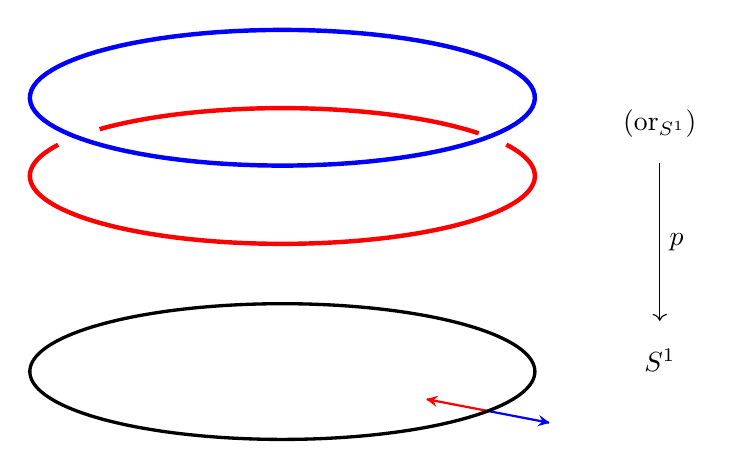
\begin{tikzpicture}
   \begin{axis}[
 view={-20}{-20},
 zmax=80,
  xmax=2,
   ymax=2,
 height=12cm,
 clip=false,hide axis
]
\addplot3+[domain=0.7:1,samples=100,samples y=0,red,no marks,thick,{stealth}-] 
({sin(deg(1.3))*x}, 
{cos(deg(1.3))*x}, 
-50);
\addplot3+[domain=1:1.3,samples=100,samples y=0,blue,no marks,thick,-{stealth}] 
({sin(deg(1.3))*x}, 
{cos(deg(1.3))*x}, 
-50);
\addplot3+[domain=0:2*pi,samples=500,samples y=0,black,no marks,very thick] 
({sin(deg(x))}, 
{cos(deg(x))}, 
-50);
\addplot3+[domain=-1.7:2.4,samples=100,samples y=0,red,no marks,ultra thick] 
({sin(deg(x))}, 
{cos(deg(x))}, 
0);
\addplot3+[domain=0:2*pi,samples=100,samples y=0,blue,no marks,ultra thick] 
({sin(deg(x))}, 
{cos(deg(x))}, 
20);
\addplot3+[domain=2.6:4.3,samples=100,samples y=0,red,no marks,ultra thick,solid] 
({sin(deg(x))}, 
{cos(deg(x))}, 
0);
\end{axis}
\draw (10,6) node{$\Spe(\mathrm{or}_{S^1})$};
\draw (10,3) node{$S^1$};
\draw[->] (10,5.5) -- (10,3.5) node[midway, right]{$p$};
\end{tikzpicture}

%% orientation_cover_of_M (Poincare_duality-3.png)
 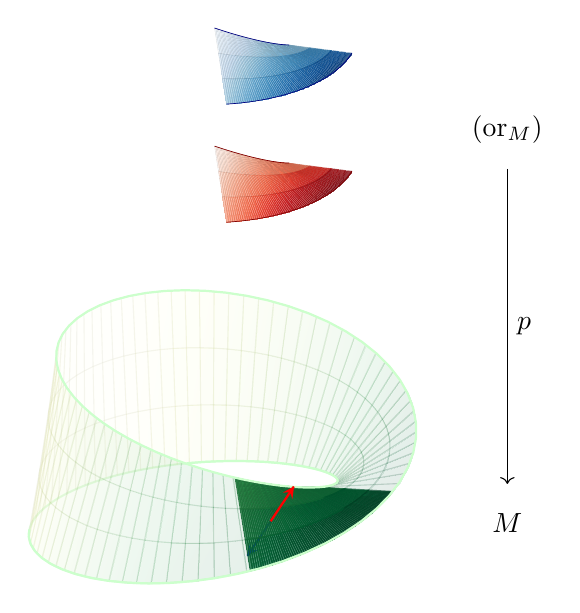
\begin{tikzpicture}
 \begin{scope}[xshift=3cm, yshift=-1.5cm, scale=.3]
    \begin{axis}[
    hide axis,
    view = {40}{40},
    colormap/Reds
    ]
    \addplot3 [
    surf,
    shader     = faceted interp,opacity = 0.7,
    %shader = interp,
    point meta = x,
    samples    = 80,
    samples y  = 4,
    z buffer   = sort,
    domain     = -50:10,
    y domain   =-0.5:0.5
    ] (
    {(1+0.5*y*cos(x/2)))*cos(x)},
    {(1+0.5*y*cos(x/2)))*sin(x)},
    {0.5*y*sin(x/2)}
    );
    \addplot3 [color=red!50!black,thick,    
    domain     = -50:10,samples y=0,samples=100,
    ] (
    {(1+0.5*0.5*cos(x/2)))*cos(x)},
    {(1+0.5*0.5*cos(x/2)))*sin(x)},
    {0.5*0.5*sin(x/2)}
    );
    \addplot3 [color=red!50!black,thick,    
    domain     = 310:370,samples y=0,samples=100,
    ] (
    {(1+0.5*0.5*cos(x/2)))*cos(x)},
    {(1+0.5*0.5*cos(x/2)))*sin(x)},
    {0.5*0.5*sin(x/2)}
    );
    \end{axis}
    \end{scope}
    \begin{scope}[xshift=3cm, yshift=0cm, scale=.3]
    \begin{axis}[
    hide axis,
    view = {40}{40},
    colormap/Blues
    ]
    \addplot3 [
    surf,
    shader     = faceted interp,opacity = 0.7,
    %shader = interp,
    point meta = x,
    samples    = 80,
    samples y  = 4,
    z buffer   = sort,
    domain     = -50:10,
    y domain   =-0.5:0.5
    ] (
    {(1+0.5*y*cos(x/2)))*cos(x)},
    {(1+0.5*y*cos(x/2)))*sin(x)},
    {0.5*y*sin(x/2)}
    );
    \addplot3 [color=blue!50!black,thick,    
    domain     = -50:10,samples y=0,samples=100,
    ] (
    {(1+0.5*0.5*cos(x/2)))*cos(x)},
    {(1+0.5*0.5*cos(x/2)))*sin(x)},
    {0.5*0.5*sin(x/2)}
    );
    \addplot3 [color=blue!50!black,thick,    
    domain     = 310:370,samples y=0,samples=100,
    ] (
    {(1+0.5*0.5*cos(x/2)))*cos(x)},
    {(1+0.5*0.5*cos(x/2)))*sin(x)},
    {0.5*0.5*sin(x/2)}
    );
    \end{axis}
    \end{scope}
    \begin{scope}[yshift=-7cm]
    \begin{axis}[
    hide axis,
    view = {40}{40},
    colormap/YlGn
    ]
    \addplot3 [color=green!10,thick,    
    domain     = 360:720,samples y=0, samples=80,
    ] (
    {(1+0.5*0.5*cos(x/2)))*cos(x)},
    {(1+0.5*0.5*cos(x/2)))*sin(x)},
    {0.5*0.5*sin(x/2)}
    );
    \addplot3 [color=blue,thick,    
    domain     = 0:-.1,samples y=0,samples=100,-{stealth}
    ] (
    {cos(30)+x},
    {sin(-30)+x},
    {x}
    );
    \addplot3 [
    surf,
    shader     = faceted interp,opacity = 0.1,
    %shader = interp,
    point meta = x,
    samples    = 80,
    samples y  = 4,
    z buffer   = sort,
    domain     = 0:360,
    y domain   =-0.5:0.5
    ] (
    {(1+0.5*y*cos(x/2)))*cos(x)},
    {(1+0.5*y*cos(x/2)))*sin(x)},
    {0.5*y*sin(x/2)}
    );
    \addplot3 [
    surf,
    shader     = faceted interp,opacity = 0.7,
    %shader = interp,
    point meta = x,
    samples    = 80,
    samples y  = 4,
    z buffer   = sort,
    domain     = -40:10,
    y domain   =-0.5:0.5
    ] (
    {(1+0.5*y*cos(x/2)))*cos(x)},
    {(1+0.5*y*cos(x/2)))*sin(x)},
    {0.5*y*sin(x/2)}
    );
    \addplot3 [color=green!20,thick,    
    domain     = -140:497.5,samples y=0,samples=100,
    ] (
    {(1+0.5*0.5*cos(x/2)))*cos(x)},
    {(1+0.5*0.5*cos(x/2)))*sin(x)},
    {0.5*0.5*sin(x/2)}
    );
    \addplot3 [color=red,thick,    
    domain     = 0:.1,samples y=0,samples=100,-{stealth}
    ] (
    {cos(30)+x},
    {sin(-30)+x},
    {x}
    );
    \end{axis}
    \end{scope}
    \draw (7,0) node{$\Spe(\mathrm{or}_M)$};
    \draw (7,-5) node{$M$};
    \draw[->] (7,-.5) -- (7,-4.5);
    \draw (7,-2.5) node[right]{$p$};
 \end{tikzpicture}